\documentclass{report}
\usepackage{graphicx} % Required for inserting images
\usepackage[left=2cm, right=2cm, top=2cm, bottom=2cm]{geometry}
\usepackage{amsmath}
\usepackage{mathtools}
\usepackage[utf8]{inputenc}
\usepackage{amssymb}
\usepackage{amsthm}
\usepackage{url}
\usepackage{hyperref}
\usepackage{xcolor}
\usepackage{enumitem}
\usepackage{lineno}

\setlength{\oddsidemargin}{0cm}
\setlength{\evensidemargin}{0cm}
\setlength{\topmargin}{0cm}
\setcounter{section}{-1}
\title{Mathematik für Informatikstudiengänge II}
\date{}

\hypersetup{
	colorlinks=true,
	linkcolor=teal,
	filecolor=magenta,      
	urlcolor=cyan,
}

\newcommand*\conj[1]{\bar{#1}}
\newcommand*\mean[1]{\bar{#1}}
\newcommand\myeq{\stackrel{\mathclap{\normalfont\mbox{IV}}}{=}}
\newcommand\griv{\stackrel{\mathclap{\normalfont\mbox{IV}}}{>}}
\newcommand\phut{\stackrel{\mathclap{\normalfont\mbox{^}}}{P}}

% Da fängt's wieder an

\begin{document}
	\maketitle
	\tableofcontents
	\newpage
	\section{Der Euklidische Raum}
		Ein euklidische Raum ist ein spezieller Vektorraum, der als $\mathbb{R}^n$ dargestellt werden kann. \textcolor{gray}{Beispiele wären also eine Ebene für $n=2$ oder der 3-dimensionale Raum, in dem wir leben mit $n=3$}. Diese speziellen Vektorräume sind praktisch, wie wir gleich sehen werden:\\
		\subsection{Standart-Skalarprodukt}
			Dieses Skalarprodukt kann schon aus der Schule bekannt sein, wird aber allgemein formuliert als:
			\begin{equation}
				\langle x, y \rangle = x_1 \cdot y_1 + \dots + x_n \cdot y_n
			\end{equation}
			Diese eckigen Klammern sind eine mögliche Schreibweise für das Skalarprodukt.
		\subsubsection{Beispiel:}
			Sei \begin{equation*} x = \begin{bmatrix}
				3 \\ 1 \\ 6 \\ -1 \\
			\end{bmatrix} \mbox { und }y = \begin{bmatrix}
			-2 \\ 0 \\ -3 \\ 1 \\
			\end{bmatrix}\end{equation*} \\
			Dann lässt sich das Skalarprodukt berechnen als:\\
			\begin{equation*} \langle x, y \rangle = 3 \cdot -2 + 1 \cdot 0 + 6 \cdot -3 + -1 \cdot 1 =  -25 \end{equation*}
			\subsubsection{Anmerkung zur Positiv-Definitheit}
				\textcolor{gray}{Das Skalarprodukt kann grundsätzlich auch negativ sein. Allerdings kann das Skalarprodukt grob vereinfacht veranschaulicht werden als die Fläche des Parallelogramms, dass von einem Vektor und dem anderen noch um 90 Grad gedrehten Vektor aufgespannt wird. Eine Fläche hat natürlich einen nicht-negativen Flächeninhalt, daher kann bei der Interpretation des Skalarprodukts manchmal der Betrag sinnvoller sein.}
			\subsubsection{Ausmultiplizieren im Skalarprodukt}
				Hier noch eine weitere Umformung, die sich im Skalarprodukt nutzen lassen. Hier sind $x, y, z$ Vektoren und $s, t$ Skalare (Zahlen):
				\begin{equation}
					\langle sx + ty, z \rangle = s\langle x, z \rangle + t\langle y, z \rangle
				\end{equation}
		\subsection{Norm eines Vektors}
			Der Norm eines Vektors lässt sich verstehen als die Länge dieses Vektors. Wer sich hier noch an die Schuldefinition erinnert ($\sqrt{x_1^2+x_2^2+\dots+x_n^2}$) wird nachvollziehen können, dass diese Formel mit dem gerade eingeführten Skalarprodukt noch etwas formalisiert werden kann:
			\begin{equation}
				\left\lVert x \right\rVert = \sqrt{\langle x, x \rangle}
			\end{equation}
			In der Vorlesung wurde noch eine weitere Gleichung eingeführt, die an die erste binomische Formel erinnert:
			\begin{equation}
					\left\lVert sx + ty \right\rVert^2 = s^2\left\lVert x \right\rVert^2 + 2st\langle x, y \rangle + t^2 \left\lVert y \right\rVert^2
			\end{equation}
		\subsection{Cauchy-Schwarz-Ungleichung}
			Diese Ungleichung besagt:
			\begin{equation}
				\langle x, y \rangle \leq \left\lVert x \right\rVert \cdot \left\lVert y \right\rVert
			\end{equation}	
			\textcolor{gray}{Anschauliche Begründung: Das Skalarprodukt (links) gibt den Flächenanhalt des Parallelogramms an, dass von einem Vektor und dem anderen noch um 90 Grad gedrehten Vektor aufgespannt wird. Das Produkt der Längen der Vektoren (rechts) kann z.B. als Flächeninhalt eines Rechtecks verstanden werden, bei dem die Seiten eben x und y sind.\\
			Die Ungleichung sagt also aus, dass der Flächeninhalt dieses Rechtecks immer mindestens so groß sein wird wie der des Parallelogramms.}
		\subsection{Dreiecksungleichung}
			Diese Ungleichung besagt:
			\begin{equation}
				\left\lVert x+y \right\rVert \leq \left\lVert x \right\rVert + \left\lVert y \right\rVert
			\end{equation}
			\textcolor{gray}{Anschauliche Begründung: Die Norm gibt immer die Länge des Vektors an. Die Länge der beiden Vektoren (rechts) addiert ist also immer mindestens so lang wie der Vektor x+y. Der Vektor x+y entsteht, indem man diese beiden Vektoren aneinander hängt. Solange die beiden Vektoren nicht in die gleiche Richtung zeigen, werden diese Vektoren ein Dreieck bilden, also ist der Abstand zwischen Anfang und Ende der beiden aneinandergehängten Pfeile  kürzer als die Länge beider Pfeile.}
		\subsection{Gram-Schmidt-Orthogonalisierung}
			Dieses Verfahren kann angewendet werden, um aus einer Basis eines Vektorraums eine Orthogonalbasis zu machen, also eine Basis, in der alle Basisvektoren rechtwinklig zueinander stehen. 
			\textcolor{gray}{Eine Ebene kann z.B. durch zwei Vektoren, die in der Ebene liegen, angegeben werden. Es kann aber manchmal sinnvoll sein, stattdessen zwei Vektoren zu haben, die zusätzlich noch rechtwinklig zueinander stehen}
		\subsubsection{Beispiel}
			Anstatt komplexer Definitionen gibt es jetzt einfach direkt ein Zahlenbeispiel: Sei die Basis des Vektorraums\\
			\begin{equation*}
				v_1 = \begin{bmatrix} 1 \\ 2 \\ 0 \\ 0 \\ \end{bmatrix}, 
				v_2 = \begin{bmatrix} 10 \\ 0 \\ 5 \\ 0 \\ \end{bmatrix}, 
				v_3 = \begin{bmatrix} 1 \\ 1 \\ 0 \\ 1 \\ \end{bmatrix}, 
			\end{equation*}
			Wir wollen jetzt dazu ein $w_1$, $w_2$, $w_3$ finden: \\
			\textbf{Schritt 1:}
			\begin{equation*} w_1 = v_1 = \begin{bmatrix} 1 \\ 2 \\ 0 \\ 0 \\ \end{bmatrix} \end{equation*}
			\textbf{Schritt 2:}\\
			Hier wird's etwas komplizierter:
			\begin{eqnarray*} w_2 &=& v_2 - \frac{\langle v_2, w_1 \rangle}{\langle w_1, w_1 \rangle} \cdot w_1 \\
				&=& \begin{bmatrix} 10 \\ 0 \\ 5 \\ 0 \\ \end{bmatrix} - \frac{(10 \cdot 1 + 0 \cdot 2 + 5 \cdot 0 + 0 \cdot 0)}
				{(1 \cdot 1 + 2 \cdot 2 + 0 \cdot 0 + 0 \cdot 0)} \cdot \begin{bmatrix} 1 \\ 2 \\ 0 \\ 0 \\ \end{bmatrix} \\
				&=& \begin{bmatrix} 10 \\ 0 \\ 5 \\ 0 \\ \end{bmatrix} - 
				\frac{10}{5} \cdot \begin{bmatrix} 1 \\ 2 \\ 0 \\ 0 \\ \end{bmatrix} \\
				&=& \begin{bmatrix} 8 \\ -4 \\ 5 \\ 0 \\ \end{bmatrix}
			\end{eqnarray*}
			\textbf{Schritt 3:}\\
			\begin{eqnarray*}
				w_3 &=& v_3 - \frac{\langle v_3, w_1 \rangle}{\langle w_1, w_1 \rangle} \cdot w_1 - \frac{\langle v_3, w_2 \rangle}{\langle w_2, w_2 \rangle} \cdot w_2\\
				&=& \begin{bmatrix} 1 \\ 1 \\ 0 \\ 1 \\ \end{bmatrix} - \frac35 \cdot \begin{bmatrix} 1 \\ 2 \\ 0 \\ 0 \\ \end{bmatrix} - \frac4{105} \cdot \begin{bmatrix} 8 \\ -4 \\ 5 \\ 0 \\ \end{bmatrix} \\
				&=& \begin{bmatrix} \frac2{21} \\ -\frac{1}{21} \\ -\frac4{21} \\ 1 \\ \end{bmatrix}
			\end{eqnarray*}
			Wir dürfen auch jederzeit unser neues $w$ skalieren, also multipliziere ich noch $w_3$ mit 21, damit das Ergebnis etwas simpler wird:\\
			\begin{equation*}
				w_3 =  \begin{bmatrix} 2 \\ -1 \\ -4 \\ 21 \\ \end{bmatrix}
			\end{equation*}
			\textbf{Schritt 4:}
			Kontrolle der Ergebnisse. Jetzt muss für jedes Paar von neuen Vektoren das Skalarprodukt 0 sein:
			\begin{eqnarray*}
				\langle w_1, w_2 \rangle &=& 0 \\
				\langle w_1, w_3 \rangle &=& 0 \\
				\langle w_2, w_3 \rangle &=& 0
			\end{eqnarray*}
			Wenn hier überall 0 rauskommt, war die Rechnung vorher korrekt. Die Orthogonalbasis ist hier also:
			\begin{equation*}
				w_1 = \begin{bmatrix} 1 \\ 2 \\ 0 \\ 0 \\ \end{bmatrix}, 
				w_2 = \begin{bmatrix} 8 \\ -4 \\ 5 \\ 0 \\ \end{bmatrix}, 
				w_3 = \begin{bmatrix} 2 \\ -1 \\ -4 \\ 21 \\ \end{bmatrix}
			\end{equation*}
		\subsection*{Orthonomalbasis}
			Eine Orthonomalbasis ist eine Orthogonalbasis, bei der zusätzlich die Norm aller Basisvektoren gleich 1 ist.\\
			\textcolor{gray}{Zusätzlich zu dem rechten Winkel der Vektoren müssen die jetzt auch noch die Länge 1 haben.}\\
			Dazu wird jeder Vektor $w$ durch seinen Norm geteilt.
			\begin{equation*}
				z_i = \frac{1}{\left\lVert w_i \right\rVert} \cdot w_i
			\end{equation*}
			\subsubsection*{Beispiel}
				Hier nehmen wir noch einmal die Orthogonalbasis aus dem vorherigen Beispiel und wandeln sie in eine Orthonormalbasis um.
				\begin{equation*}
					w_1 = \begin{bmatrix} 1 \\ 2 \\ 0 \\ 0 \\ \end{bmatrix}, 
					w_2 = \begin{bmatrix} 8 \\ -4 \\ 5 \\ 0 \\ \end{bmatrix}, 
					w_3 = \begin{bmatrix} 2 \\ -1 \\ -4 \\ 21 \\ \end{bmatrix}
				\end{equation*}
				\begin{eqnarray*}
					z_1 &=& \frac{1}{\left\lVert w_1 \right\rVert} \cdot w_1 = \frac1{\sqrt{5}} \cdot \begin{bmatrix} 1 \\ 2 \\ 0 \\ 0 \\ \end{bmatrix} = \begin{bmatrix} \frac1{\sqrt{5}} \\ \frac2{\sqrt{5}} \\ 0 \\ 0 \\ \end{bmatrix} \\
					z_2 &=& \frac{1}{\left\lVert w_2 \right\rVert} \cdot w_2 = \frac1{\sqrt{105}} \cdot \begin{bmatrix} 8 \\ -4 \\ 5 \\ 0 \\ \end{bmatrix} = \begin{bmatrix} \frac8{\sqrt{105}} \\ -\frac4{\sqrt{105}} \\ \frac5{\sqrt{105}} \\ 0 \\ \end{bmatrix} \\
					z_3 &=& \frac{1}{\left\lVert w_3 \right\rVert} \cdot w_3 = \frac1{\sqrt{462}} \cdot \begin{bmatrix} 2 \\ -1 \\ -4 \\ 21 \\ \end{bmatrix} = \begin{bmatrix} \frac2{\sqrt{462}} \\ -\frac1{\sqrt{462}} \\ -\frac4{\sqrt{462}} \\ \frac{21}{\sqrt{462}} \\ \end{bmatrix}
				\end{eqnarray*}
				Es ergibt sich also die Orthonormalbasis
				\begin{equation*}
					z_1 = \begin{bmatrix} \frac1{\sqrt{5}} \\ \frac2{\sqrt{5}} \\ 0 \\ 0 \\ \end{bmatrix},
					z_2 = \begin{bmatrix} \frac8{\sqrt{105}} \\ -\frac4{\sqrt{105}} \\ \frac5{\sqrt{105}} \\ 0 \\ \end{bmatrix}, 
					z_3 = \begin{bmatrix} \frac2{\sqrt{462}} \\ -\frac1{\sqrt{462}} \\ -\frac4{\sqrt{462}} \\ \frac{21}{\sqrt{462}} \\ \end{bmatrix}
				\end{equation*}
			\subsection{Lemma zur Rechtwinkligkeit (19.6)}
				In einem Teilraum $U$ gibt immer ein $u_0 \in U$ sodass für jedes $v \in \mathbb{R}$ ein $v'$ existiert, sodass $v = u_0 + v$ und $\langle u, v'\rangle = 0 \forall u \in U$ gilt.\\
				\textcolor{gray}{Veranschaulichung: Sei der Vektorraum 3-dimensional und der Teilraum $U$ eine Ebene, z.B der Boden. Dann sagt dieses Lemma aus, dass jeder Punkt in diesem "Raum" auch dargestellt werden kann als ein Vektor auf dem Boden plus ein dazu senkrecht stehender Vektor}
		\subsection{Methode der kleinsten Quadrate}
			Hierbei handelt es sich um eine Methode, mit der eine Ausgleichsfunktion durch eine Anzahl von Datenpunkten gefunden wird. Im folgenden Beispiel suchen wir eine Ausgleichsgerade, also eine lineare Funktion, die so nah wie möglich an allen Datenpunkten liegt.
			\subsubsection{Beispiel}
				Seien folgende Werte für $x, y$ gegeben:\\
				\begin{center} \begin{tabular}{c|c|c|c|c|c}
					x & 0 & 1 & 2 & 3 & 4\\ \hline
					y & 2 & 0 & 1 & 2 & 3\\
				\end{tabular} \end{center}
				Wir wollen hier jetzt eine Ausgleichsgerade durch legen: \\Diese Ausgleichsgerade sieht allgemein so aus:
				\begin{equation*}
						f(x) = p_0 + p_1 \cdot x
				\end{equation*}
				Diese Werte wollen wir nun in ein Gleichungssystem umschreiben:
				\begin{eqnarray*}
					p_0 + 0 \cdot p_1 &=& 2 \\ 
					p_0 + 1 \cdot p_1 &=& 0 \\ 
					p_0 + 2 \cdot p_1 &=& 1 \\
					p_0 + 3 \cdot p_1 &=& 2 \\
					p_0 + 4 \cdot p_1 &=& 3
				\end{eqnarray*}
				Dieses Gleichungssystem wandeln wir nun in eine Gleichung mit Matrizen um:
				\begin{equation*}
					\begin{bmatrix}
						1 & 0 \\ 1 & 1 \\ 1 & 2 \\ 1 & 3 \\ 1 & 4 \\
					\end{bmatrix} \cdot \begin{bmatrix}
					p_0 \\ p_1
					\end{bmatrix} = \begin{bmatrix} 2 \\ 0 \\ 1 \\ 2 \\ 3 \end{bmatrix}
				\end{equation*}
				Nun multiplizieren wir beide Seiten mit der transponierten Koeffizientenmatrix:
				\begin{eqnarray*}
					A^T \cdot \begin{bmatrix}
						1 & 0 \\ 1 & 1 \\ 1 & 2 \\ 1 & 3 \\ 1 & 4 \\
					\end{bmatrix} \cdot \begin{bmatrix}
						p_0 \\ p_1
					\end{bmatrix} &=& A^T \cdot \begin{bmatrix} 2 \\ 0 \\ 1 \\ 2 \\ 3 \end{bmatrix} \\
					\begin{bmatrix}
						1 & 1 & 1 & 1 & 1 \\
						0 & 1 & 2 & 3 & 4 \\
					\end{bmatrix}\cdot \begin{bmatrix}
						1 & 0 \\ 1 & 1 \\ 1 & 2 \\ 1 & 3 \\ 1 & 4 \\
					\end{bmatrix} \cdot \begin{bmatrix}
						p_0 \\ p_1
					\end{bmatrix} &=& \begin{bmatrix}
					1 & 1 & 1 & 1 & 1 \\
					0 & 1 & 2 & 3 & 4 \\
					\end{bmatrix} \cdot \begin{bmatrix} 2 \\ 0 \\ 1 \\ 2 \\ 3 \end{bmatrix} \\
					\begin{bmatrix}
						5 & 10 \\ 10 & 30 \\
					\end{bmatrix} \cdot \begin{bmatrix}
					p_0 \\ p_1
					\end{bmatrix} &=& \begin{bmatrix} 8 \\ 20 \end{bmatrix}
				\end{eqnarray*}
				Diese Gleichung können wir jetzt noch mittels Gauß lösen:
				\begin{eqnarray*}
					\begin{bmatrix}
						5 & 10 \\ 0 & 10 \\
					\end{bmatrix} \cdot \begin{bmatrix}
						p_0 \\ p_1
					\end{bmatrix} &=& \begin{bmatrix} 8 \\ 4 \end{bmatrix} \\
					\begin{bmatrix}
						5 & 0 \\ 0 & 10 \\
					\end{bmatrix} \cdot \begin{bmatrix}
						p_0 \\ p_1
					\end{bmatrix} &=& \begin{bmatrix} 4 \\ 4 \end{bmatrix} \\
					\begin{bmatrix}
						1 & 0 \\ 0 & 1 \\
					\end{bmatrix} \cdot \begin{bmatrix}
						p_0 \\ p_1
					\end{bmatrix} &=& \begin{bmatrix} \frac45 \\ \frac25 \end{bmatrix} \\
					p_0 = \frac45 &, & p_1 = \frac25
				\end{eqnarray*}
				Wir haben nun Werte für die beiden gesuchten Werte gefunden, also lautet die Ausgleichsgerade
				\begin{equation*}
					f(x) = \frac45 + \frac25 \cdot x
				\end{equation*}
				Das gleiche Prinzip kann auch genutzt werden, um eine Ausgleichsparabel, Ausgleichshyperbel usw. zu finden. Für ein weiteres Beispiel einer Parabel kann ich zum Beispiel \href{https://www.abi-mathe.de/buch/matrizen/methode-der-kleinsten-quadrate/}{diese Seite} hier empfehlen.
			\subsection{Lösung mit minimaler Norm (Satz 19.8)}
				Sei $L$ ein Untervektorraum eines euklidischen Raumes. In der Vorlesung ist $L$ zusätzlich der Lösungsraum eines LGS. In $L$ gibt es nun genau einen Vektor mit der kleinsten Norm.\\
				\textcolor{gray}{Sei anschaulicher der euklidische Raum nun 3-dimensional und $L$ eine 2-dimensionale Ebene. Dann sagt dieser Satz aus, dass es einen Punkt in dieser Ebene gibt, die dem Ursprung am nächsten liegt. Außerdem: der Vektor vom Ursprung auf diesen Punkt liegt orthogonal zum Lösungsraum $L$}
		\chapter{Folgen und Reihen}
			\section{Grenzwerte von Folgen}
				Funktionen sind üblicherweise definiert als $ D \rightarrow \mathbb{R}$, wobei $D \subseteq \mathbb{R}$ gilt. \textcolor{gray}{Eine Funktion bildet also eine Menge an Zahlen in $\mathbb{R}$ auf $\mathbb{R}$ ab.}\\
				Hier sind uns aus der Schule noch Polynomfunktionen, Wurzelfunktionen, Exponentialfunktionen, trigonometrische Funktionen usw. bekannt.\\
				Folgen sind nun konkrete Funktionen mit $D = \mathbb{N}_0 $, die nun auch als $f = (a_n)_{n\in\mathbb{N}_0}$ bezeichnen kann. \textcolor{gray}{Bei einer Folge wird also jeder natürlicher Zahl ein Wert zugewiesen, es gibt also ein nulltes Folgenglied, ein erstes Folgenglied usw.}
				\subsection{Definition zur Konvergenz}
					Eine Folge $f$ heißt konvergent gegen den Grenzwert $\alpha$, wenn gilt:
					\begin{equation}
						\mbox{Zu jedem } \varepsilon \in \mathbb{R}, \varepsilon > 0 \mbox{ gibt es ein } n_0 \in \mathbb{N}_0 mit \mid a_n - \alpha \mid < \varepsilon \mbox{ für alle } n \geq n_0
					\end{equation}
					\textcolor{gray}{
						Grundsätzlich: Eine Folge ist konvergent, wenn sie sich, je höher das Folgenglied, einem bestimmten Wert (Z.B. häufig 0) immer weiter annähert. Nochmal konkret zum Satz: falls eine Funktion konvertiert, gibt es bei jedem Folgenglied (ab einer bestimmten Höhe) einen Abstand zum Grenzwert, der für kein späteres Folgenglied wieder größer wird. Oder: Für jedes Folgenglied wird der Abstand zum Grenzwert geringer.}
					Ist eine Folge nicht konvergent, so ist sie stattdessen divergent. 
			\subsection{Beispiel 27.2}
				Hier fasst das Skript einige sehr gute Beispiele, an denen es eigentlich nichts hinzuzufügen gibt. Daher füge ich hier den Ausschnitt des Skripts hinzu:\\
				\begin{center} 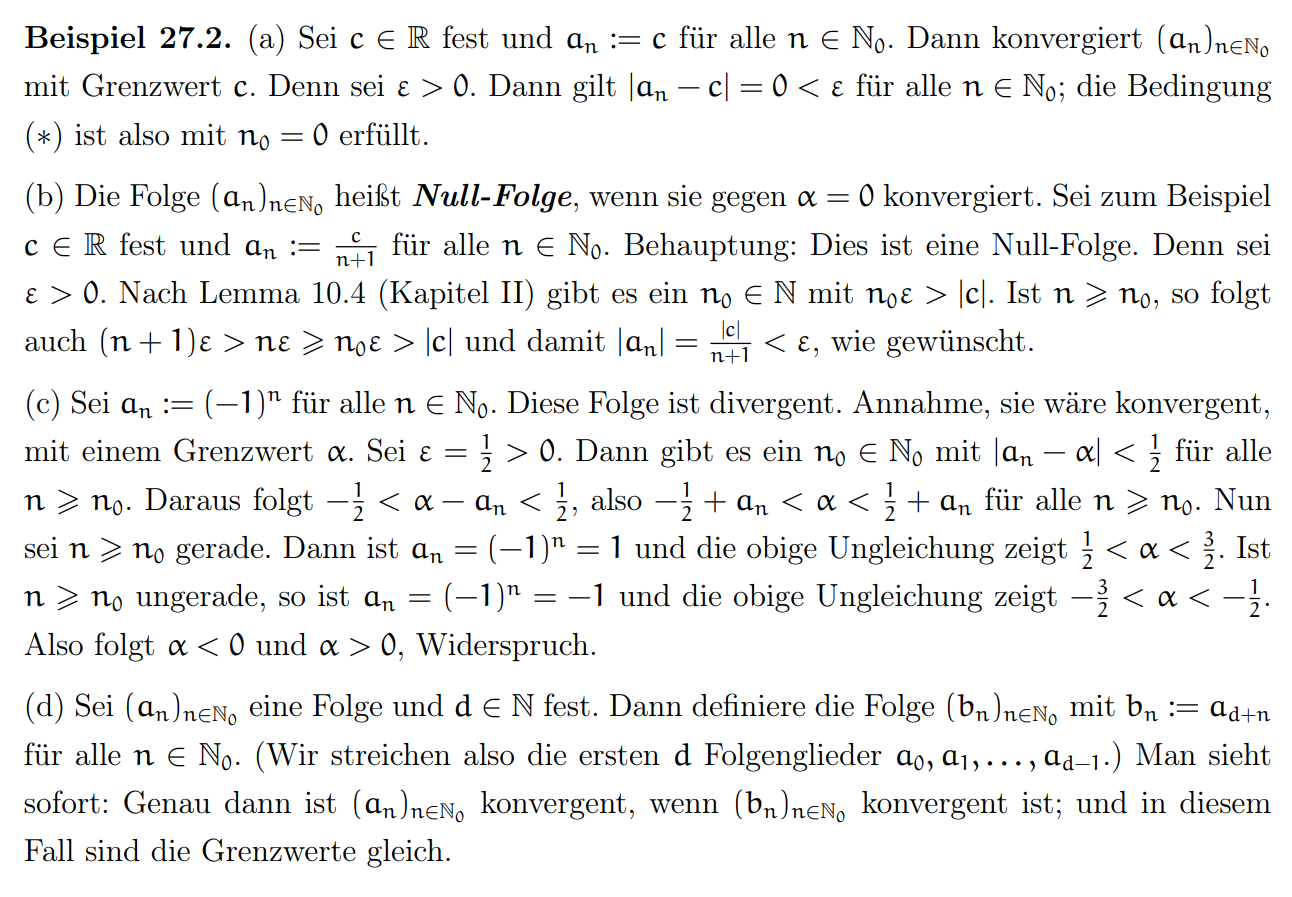
\includegraphics[width = 15cm]{pictures/Beispiel 27.2} \end{center}
			\subsubsection{Bemerkung 27.3}
				Sei eine Funktion mit $F:D \rightarrow \mathbb{R}$ mit $D = \{n \in \mathbb{N}_0 \mid n > d\}$ definiert, dann gelten die gleichen Regeln, wie vorher gezeigt. \\
				\textcolor{gray}{Sollte die Funktion erst für höhere Werte definiert werden, Z.B. ist $\sqrt{x-3}$ ist nur für $x \geq 3$ definiert. Auch diese Folgen sind genauso konvergent oder divergent, weil man sie "auf den Nullpunkt verschieben kann" }
			\subsubsection{Lemma 27.4 zu konvergenten Folgen}
				\begin{enumerate}[label=(\alph*)]
					\item Der Grenzwert $\alpha$ einer konvergenten Folge ist eindeutig.
					\textcolor{gray}{Eine konvergente Folge nähert sich einem Grenzwert beliebig genau an. Da kann es nicht noch einen weiteren Grenzwert der Folge geben.}
					\item Die Werte einer Folge sind nach oben und unten beschränkt.
					\textcolor{gray}{Eine konvergente Folge konvergiert gegen einen Grenzwert und geht daher nicht beliebig weit in eine Richtung, ist also begrenzt.}
				\end{enumerate}
			\subsubsection{Lemma 27.5 - Cauchy}
				\textit{$
					\mbox{Sei } (a_n)_{n\in\mathbb{N}_0} \mbox{ eine Folge reeller Zahlen. Ist diese Folge konvergent,  so gibt es zu jedem } \varepsilon > 0 \mbox{ ein } n_0 \in \mathbb{N}_0 \mbox{ mit } |a_n - a_m| < \varepsilon \mbox{ für alle } n \geq m \neq n_0
				$}\\
				\textcolor{gray}{Dieser Satz über konvergierende Folgen sagt aus, dass der Abstand zwischen Funktionswerten beliebig klein werden. Für jedes positives $\varepsilon$ werden die Abstände zwischen den Folgengliedern beliebig klein, und eben auch kleiner als $\varepsilon$.}
			\subsubsection{Satz 27.6 - Einschließungs-Kriterium}
				\textit{Seien $f_a, f_b, f_c$ Folgen, wobei sowohl $f_a$ als auch $f_b$ gegen $\alpha$ konvergieren. Wenn nun auch $a \leq c \leq b$ für jedes Folgenglied gilt, konvergiert auch $f_c$ gegen $\alpha$}.\\
				\textcolor{gray}{Die Folge $f_c$ ist zwischen $f_a$ und $f_b$ "eingeklemmt". Damit muss $f_c$ auch am gleichen Grenzwert ankommen. Dieser Satz ist vor allem dafür wichtig, den Grenzwert von Folgen zu bestimmen. Wenn man für eine Folge zwei weitere Folgen, eine mit größeren Funktionswerten und eine mit kleineren Funktionswerten, die beide den gleichen Grenzwert haben.}
			\subsubsection{27.7 - $c^n$}
				Generell gilt: $c^n$ ist genau dann eine Nullfolge, wenn $|c| < 1$ gilt. \\
				\textcolor{gray}{Eine Exponentialfunktion geht entweder gegen 0, oder divergiert}
			\subsubsection{27.8 - Grenzwert-Regeln}
				Gegeben seien konvergente Folgen $(a_n)_{n\in\mathbb{N}_0}$ und $(b_n)_{n\in\mathbb{N}_0}$ in $\mathbb{R}$. Sei $\alpha := \displaystyle\lim_{n\to\infty}(a_n)$ und $\beta:= \displaystyle\lim_{n\to\infty}(b_n)$
				\begin{enumerate}[label=(\alph*)]
					\item Die Folge $c_n := ra_n + sb_n$ konvergiert gegen $r\alpha+s\beta$
					\item Die Folge $c_n := a_n \cdot b_n$ konvergiert gegen $\alpha \cdot \beta$
					\item Die Folge $c_n := \frac{a_n}{b_n}$ konvergiert gegen $\frac{\alpha}{\beta}$, solange $b_n \neq 0$ und $\beta \neq 0$
					\item Gibt es ein $n_0 \in \mathbb{N}_0$ mit $a_n \leq b_n$ für alle $n \geq n_0$, so ist auch $\alpha \leq \beta$
					\textcolor{gray}{Wenn die Funktion $a$ über $b$ liegt, ist der Grenzwert von $a$ auch über dem Grenzwert von $b$}
				\end{enumerate}
		\subsubsection{27.11 - konkretes Beispiel zum Grenzwert}
			Wir wollen den Grenzwert von $a_n$ bestimmen: 
			\begin{equation*}
				a_n = \frac{2n^2 + 3n + 5}{4n^2+5n+1}
			\end{equation*}
			Nun kürzen wir mit der höchsten Potenz, hier also $n^2$:
			\begin{equation*}
				\frac{2n^2 + 3n + 5}{4n^2+5n+1} = \frac{2 +\frac3n + \frac5{n^2}}{4 + \frac5n + \frac1{n^2}} \rightarrow \frac{2 + 0 + 0}{4 + 0 + 0} = \frac12
			\end{equation*}
			jeder Bruch der Form $\frac{k}{n^l}$ mit $l\geq 1$ geht für $n \to \infty$ gegen 0, daher kann man diese mit 0 ersetzen.
		\subsubsection{27.12 - Monotonie}
			 \begin{center}
			 	$\mathrm{f~heißt}\quad
			 	\begin{Bmatrix}
			 		\text{monoton wachsend} \\
			 		\text{streng monoton wachsend} \\
			 		\text{monoton fallend} \\
			 		\text{streng monoton fallend}
			 	\end{Bmatrix},\quad\mathrm{falls}\quad
			 	\begin{Bmatrix}
			 		\mathrm{f(x)\leqslant f(y)} \\
			 		\mathrm{f(x)<f(y)} \\
			 		\mathrm{f(x)\geqslant f(y)} \\
			 		\mathrm{f(x)>f(y)}
			 	\end{Bmatrix}$
			 \end{center}
			 Beispiele:
			 \begin{itemize}
			 	\item $x^2$ hat keine vollständige Monotonie
			 	\item $x^3$ ist monoton wachsend
			 	\item $-x$ ist streng monoton fallend
			 	\item $e^x$ ist streng monoton wachsend
			 \end{itemize}
		\subsubsection{Monotonie-Prinzip}
			Eine monoton wachsende und beschränkte Folge ist konvergent\\
			\\
			\textcolor{gray}{Eine Folge, dessen Werte nur nach "oben gehen", aber nach oben beschränkt ist, muss zu dieser Grenze konvergieren}
		\subsubsection{bestimmte Divergenz}
			Eine Folge ist bestimmt divergent gegen $\infty$, wenn die Werte der Folge ab einem bestimmten Folgenglied immer größer werden. \textcolor{gray}{Die Werte von $x^2$ werden immer größer und sind nicht beschränkt. $x^2$ divergiert also bestimmt gegen $\infty$}
			Eine Folge kann auf die gleiche Weise bestimmt divergent gegen $-\infty$ sein.
		\subsubsection{Lemma 27.17 - zur Divergenz}
			Ist eine Folge $a_n$ divergent gegen $\pm \infty$, so konvergiert $\frac1{a_n}$ gegen 0\\
	\section{Unendliche Reihen}
		\subsection{Definition}
		Für eine Folge $a_n$ ist $A_n$ mit $A_n := \sum_{k=0}^n ak$ die Reihe, wobei jedes $A_n$ eine Partialsumme darstellt.\\
		\textcolor{gray}{Die Reihe ist also die Summe aller Folgenglieder. Ist die Folge also $a_n = 1$ für alle $a_n$, so ist die Reihe dazu $A_n = n$}
		\subsection{geometrische Reihe}	
		Eine geometrische Reihe ist eine Reihe über eine exponentielle Folge. Hier gilt für eine Folge $a_n = c^n$, dass die Reihe genau dann konvergiert, wenn $|c| \leq 1$ gilt. Sonst würde die Reihe divergieren.
		Falls die Reihe konvergiert, gilt:\\
		\begin{equation}
			\displaystyle\sum_{n=0}^{\infty} c^n = lim_{n\to\infty}(A_n) = \frac1{1-c}
		\end{equation}
		Mit dieser Formel kann man den Grenzwert einer geometrischen Reihe bestimmen.
		\subsection{Lemma 28.3 zur Konvergenz von Reihen}
		Konvergiert eine Reihe $A_n$, so ist $a_n$ eine Nullfolge.\\
		\textcolor{gray}{Wenn die Summe der Folgenglieder sich irgendwann nicht mehr groß ändert, dürfen die Folgenglieder selbst auch nicht mehr groß sein.}
		\subsection{Bemerkung zum Beginn der Summe}
		Es ist für die Konvergenzbetrachtung einer Reihe egal, ab welchem Index die Summe genommen wird. So gilt für $\sum_{k=0}^{n}a_n$ die gleiche Konvergenz wie für $\sum_{k=1000}^n a_n$. Genau wenn eine dieser Reihen konvergiert, konvergiert auch die andere. Achtung! Die Grenzwerte selbst müssen nicht gleich sein, lediglich deren Existenz.
		\subsection{$a_n = \frac1n$}
			Die Reihe über $a_n = \frac1n$ konvergiert nicht. Der Beweis wir in der Vorlesung dargestellt, hier ist nur relevant, das wir dies als gegeben annehmen können.
		\subsection{Summenregel}
			Seihen $A_n$ und $B_n$ konvergente Reihen: So konvergiert $\sum_{k=0}^{\infty} ra_n + sb_n$ gegen $r \cdot \sum_{k=0}^{\infty} a_n + s \cdot \sum_{k=0}^{\infty} b_n$
		\subsection{Absolute Konvergenz}
			Eine Reihe $A_n$ ist genau dann \textbf{absolut Konvergent}, wenn die Reihe $\sum_{k=0}^{\infty} |a_n| $ konvergiert.\\
			Falls eine Reihe absolut konvergent ist, so ist sie auch konvergent.
		\subsection{Majoranten-Kriterium}
			Sandwich-Kriterium für Reihen: Gilt für zwei Folgen $a_n$, $b_n$ $0 \leq a_n \leq b_n$ für alle $n$, und konvergiert die Reihe über $b_n$, so konvergiert auch die Reihe über $a_n$. \\
			\textcolor{gray}{Dieser Satz folgt aus der Idee des Sandwich-Prinzips.}
			Das lässt sich auch in die andere Richtung kleiner 0 (als Minoranten-kriterium) durchführen.
		\subsection{Vollständigkeit der Grenzwerte}
			Für jedes $x\in \mathbb{R} $ gibt es eine Folge mit x als Grenzwert.
		\subsection{Cauchy-Produkt von Reihen}
			Seien $A_n$ und $B_n$ absolut konvergierende Folgen. Das Cauchy-Produkt ist die Reihe $c_n$ mit $c_n := \sum_{k=0}^{\infty} a_kb_{n-k}$ Dann ist auch $c_n$ konvergent und es gilt: 
			\begin{equation}
				\displaystyle \sum_{k=0}^{\infty} c_n = \displaystyle \sum_{k=0}^{\infty} a_n \cdot \displaystyle \sum_{k=0}^{\infty} b_n 
			\end{equation}
			\textcolor{gray}{Hier verzichte ich auf den Beweis, hierfür kann ich nur auf die Vorlesung verweisen. }
		\subsection{Leibniz-Kriterium}
			Sei $a_n$ eine Nullfolge (mit $a_n \geq 0$) die monoton fällt ($a_n \geq a_{n+1}$). Dann konvergiert die Reihe $\sum_{k=0}^{\infty} (-1)^n \cdot a_n$.\\
			\textcolor{gray}{Tatsächlich benutzen wir das eher umgekehrt. Wenn $a_n$ eine Reihe ist, die den Faktor $(-1)^n$ beinhaltet, können wir die Folge ohne diesen Faktor betrachten, und an dieser neuen Folge herausfinden, ob die Reihe über $a_n$ konvergiert.}
		\subsection{Quotienten-Kriterium}
			Sei $a_n$ eine Folge: Für genügend große $k$ muss $\mid\frac{a_{k+1}}{a_k}\mid \leq 1$ gelten, dann ist die Reihe über $a_n$ absolut konvergent.\\
			\textcolor{gray}{Dieser Satz folgt direkt aus der Bedeutung der Nullfolge für die dazugehörige Reihe. Um das Quotienten-Kriterium anzuwenden dividiert man allgemein zwei aufeinander folgende Folgenglieder durcheinander und weist nach, das der Betrag des Quotienten kleiner 1 ist.}
	\section{Potenzreihen und die Exponential-Funktion}
		
	\end{document}